\documentclass[a4paper,leqno]{article}
\usepackage[utf8]{inputenc}
\usepackage{lmodern}
\usepackage{microtype}
\usepackage[inline]{enumitem}

\usepackage{siunitx}
\usepackage{multirow}
\usepackage{subcaption}

\usepackage[english]{babel}
\usepackage[autostyle, english=british]{csquotes}
\MakeOuterQuote{"}

\usepackage{commath}
\usepackage{amsmath}
\usepackage{amsthm}
\usepackage{amssymb}
\usepackage{mathtools}

\usepackage{pgfplots}
\pgfplotsset{compat=1.11}
\usepgfplotslibrary{fillbetween}
\usetikzlibrary{patterns}

\usepackage{hyperref}

\usepackage[margin=1in]{geometry}
\usepackage{changepage}
\usepackage{titlesec}
\titleformat{\section}{\normalfont\Large\bfseries\centering}{Section~\thesection:}{1em}{}

\def\signed #1{{\leavevmode\unskip\nobreak\hfil\penalty50\hskip2em
  \hbox{}\nobreak\hfil(#1)%
  \parfillskip=0pt \finalhyphendemerits=0 \endgraf}}
\newsavebox\mybox
\newenvironment{aquote}[1]
  {\savebox\mybox{#1}\begin{quote}}
  {\signed{\usebox\mybox}\end{quote}}

% Augmented matrices.
\makeatletter
\renewcommand*\env@matrix[1][*\c@MaxMatrixCols c]{%
  \hskip -\arraycolsep
  \let\@ifnextchar\new@ifnextchar
  \array{#1}}
\makeatother

%--------grstep
% For denoting a Gauss' reduction step.
% Use as: \grstep{\rho_1+\rho_3} or \grstep[2\rho_5 \\ 3\rho_6]{\rho_1+\rho_3}
\newcommand{\grstep}[2][\relax]{%
   \ensuremath{\mathrel{
       {\mathop{\longrightarrow}\limits^{#2\mathstrut}_{
                                     \begin{subarray}{l} #1 \end{subarray}}}}}}
\newcommand{\swap}{\leftrightarrow}


\swapnumbers
\numberwithin{equation}{section}
\newtheorem{thm}[equation]{Theorem}
\newtheorem{lem}[equation]{Lemma}
\newtheorem{cor}[equation]{Corollary}
\newtheorem{prp}[equation]{Proposition}
\theoremstyle{definition}
\newtheorem{defn}[equation]{Definition}
\newtheorem{notation}[equation]{Notation}
\newtheorem{ex}[equation]{Example}
\newtheorem{exercise}[equation]{Exercise}
\newtheorem{alg}[equation]{Algorithm}
\theoremstyle{remark}
\newtheorem{rem}[equation]{Remark}

\newcommand{\df}[1]{\textbf{#1}}
\newcommand{\T}{\mathrm{T}}
\newcommand{\F}{\mathrm{F}}
\newcommand{\IndSet}{\mathbf{I}}
\DeclareMathOperator{\cis}{cis}

\title{Level Three Trigonometry}
\author{Alex Elzenaar}
\date{\today}

\begin{document}
\maketitle
\tableofcontents
\section*{Preface}
These notes present a brief overview of the trigonometry required for Level 3 Calculus. We
mainly treat the subject from a functional viewpoint.

\titleformat{\section}{\clearpage\titlerule[0.8pt]\vspace{0.5ex}\normalfont\Large\bfseries\centering}{Section~\thesection:}{1em}{}[{\titlerule[0.8pt]}]
\let\oldsection\section
\renewcommand\section{\clearpage\oldsection}
\section{Definitions}

\begin{notation}
  We will denote points by uppercase letters; the line through the points $ X $ and $ Y $ is denoted $ XY $, and the length of the
  segment between $ X $ and $ Y $ will be denoted $ \abs{XY} $. If $ O $, $ A $, and $ B $ are points, then $ \angle AOB $ denotes
  the angle that starts at the ray $ OA $ and is measured anticlockwise to the ray $ OB $.
\end{notation}

\begin{center}
  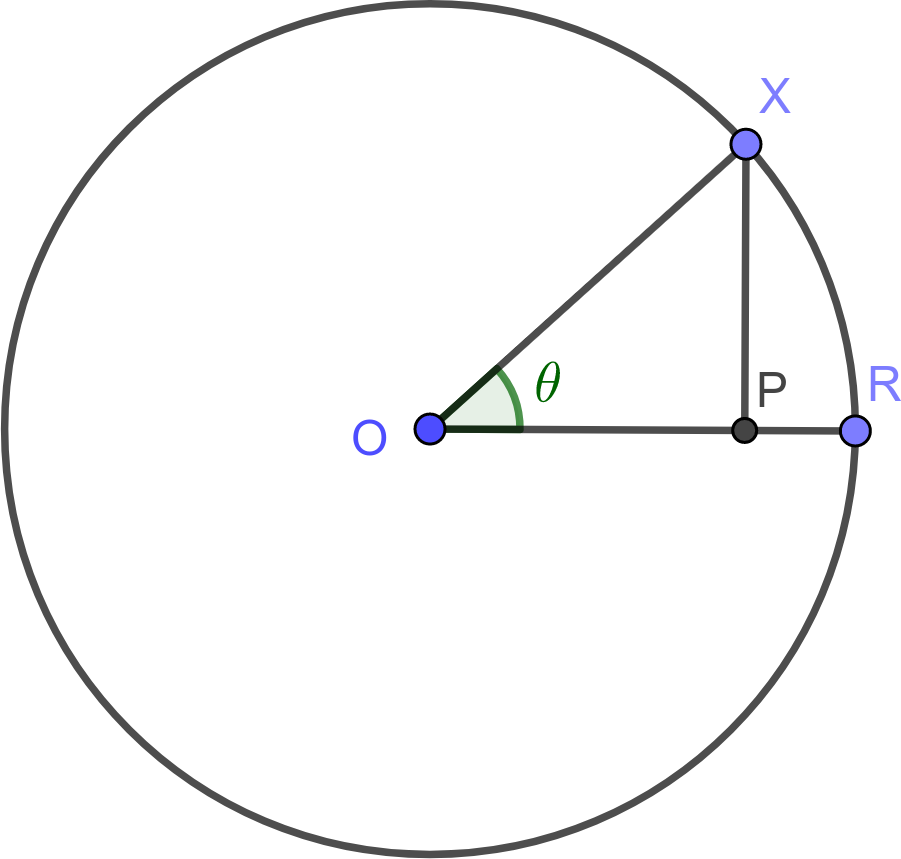
\includegraphics[width=0.3\textwidth]{fndefinitions}
\end{center}

\begin{defn}\label{defn:trig1}
  Consider a unit circle with centre $ O $ and radius $ OR $. Let $ X $ be any point on the circle, such that the angle between $ OR $ and $ OX $
  is $ \theta $ (i.e. such that the proportion of the circumference between $ R $ and $ X $ is $ \theta/2\pi $). Draw the line through $ X $,
  perpendicular to the radius $ OR $ and cutting the latter at $ P $. Then we define two functions of $ \theta $ as follows, called the \df{sine} and \df{cosine}
  functions respectively, for all $ 0 \leq \theta < \pi/2 $:-
  \begin{gather}
    \sin(\theta) = \abs{PX}\\
    \cos(\theta) = \abs{OP}.
  \end{gather}
\end{defn}

It is customary to drop the parentheses around the argument of trigonometric functions if it is a single term; for
example, $ \sin \theta $ simply means $ \sin(\theta) $. We adopt this convention whenever it is unambiguous.

It is also customary to write $ \sin^2 \theta $ in place of $ (\sin \theta)^2 $, and in general $ \sin^n \theta $
for $ (\sin \theta)^n $ whenever $ n $ is a positive integer.

Clearly, we also have $ \sin 0 = 0 $ and $ \cos 0 = 1 $.

We then extend the domains of definition of sine and cosine to the entire range $ 0 \leq \theta < 2\pi $, as follows:
\begin{equation}\label{tab:extend1}
\begin{tabular}{c|c|c|c}
  & $ \frac{\pi}{2} \leq \theta < \pi $ & $ \pi \leq \theta < \frac{3\pi}{2} $ & $ \frac{3\pi}{2} \leq \theta < 2\pi $\\\hline
  $ \sin \theta = $ & $ \sin(\pi - \theta) $ & $ -\sin(\theta - \pi)$ & $-\sin(2\pi - \theta) $\\
  $ \cos \theta = $ & $ -\cos(\pi - \theta) $ & $ - \cos (\theta - \pi) $ & $ \cos(2\pi - \theta) $.
\end{tabular}
\end{equation}

Drawing the graphs of $ y = \sin x $ (red) and $ y = \cos x $ (blue) for $ 0 \leq x < 2\pi $, we obtain the
following picture.
\begin{center}
  \fbox{\begin{tikzpicture}
    \begin{axis}[
      axis lines = center,
      ymax = 1.5, ymin = -1.5,
      xtick={1.5708, 3.14159, 4.7124, 6.28},
      xticklabels={$\frac{\pi}{2}$,$\pi$,$\frac{3\pi}{2}$,$2\pi$},
      xlabel = $ x $,
      ylabel = $ y $
    ]
      \addplot[domain = 0:2*pi, color = red] {sin(deg(x))};
      \addplot[domain = 0:2*pi, color = blue] {cos(deg(x))};
    \end{axis}
  \end{tikzpicture}}
\end{center}

Finally, we extend the domains of definition to the entire real line by declaring that for all real $ \theta $, the identities
\begin{gather}
  \sin \theta = \sin (\theta + 2n\pi)\text{ and}
  \cos \theta = \cos (\theta + 2n\pi)
\end{gather}
hold (where $ n $ is any integer). This simply implies that the graphs of the two functions repeat every $ 2\pi $; hence the graphs
as drawn above can be extended as far as we like in either direction by just making shifted copies of the bit we already drew.
\begin{center}
  \fbox{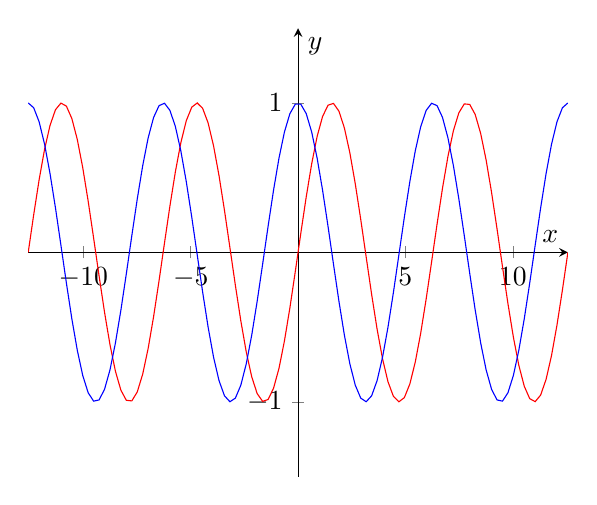
\begin{tikzpicture}
    \begin{axis}[
      axis lines = center,
      ymax = 1.5, ymin = -1.5,
      xtick={},
      xlabel = $ x $,
      ylabel = $ y $
    ]
      \addplot[domain = -4*pi:4*pi, color = red, samples=100] {sin(deg(x))};
      \addplot[domain = -4*pi:4*pi, color = blue, samples=100] {cos(deg(x))};
    \end{axis}
  \end{tikzpicture}}
\end{center}

\begin{exercise}
  Consider the unit circle again, call $ PX $ positive whenever $ X $ lies above the $ OR $ axis and negative whenever $ X $ lies below that
  axis. Then call $ OP $ positive whenever $ P $ lies on the segment $ OR $ and negative when $ P $ lies on the opposite side of $ R $. Show
  that if we define $ \sin \theta $ and $ \cos \theta $ by $ PX $ and $ OP $ respectively for all $ 0 \leq \theta < 2\pi $, keeping signs
  consistent, then the resulting functions agree with our definition above.
\end{exercise}

\begin{prp}
  The following identities always hold.
  \begin{enumerate}
    \item $ -1 \leq \sin \theta \leq 1 $ and $ -1 \leq \cos \theta \leq 1 $ for all $ \theta $.
    \item $ \sin 2n\pi = 0 $ and $ \cos 2n\pi = 1 $ for all integers $ n $.
    \item $ \sin^2 \theta + \cos^2 \theta = 1 $ for all $ \theta $.
    \item $ \sin (-\theta) = -\sin \theta $ and $ \cos (-\theta) = \cos \theta $ for all $ \theta $.
    \item $ \cos \theta = \sin (\theta + \pi/2) $.
  \end{enumerate}
\end{prp}
\begin{proof}\leavevmode
  \begin{enumerate}
    \item For $ 0 \leq \theta < \pi/2 $, the two functions are defined using the lengths $ PX $ and $ OP $ which
          are positive and always less than 1. For all other values of $ \theta $, the functions are defined in
          terms of the values on this interval and are not scaled beyond a negative sign; so both functions are
          bounded above by 1 and below by $ -1 $.
    \item $ \sin 2n\pi = \sin(0 + 2n\pi) = \sin 0 = 0 $. A similar calculation holds for cosine.
    \item When $ 0 \leq \theta < \pi/2 $, the statement follows from an application of Pythagoras' theorem
          to the right triangle $ OPX $. When $ \pi/2 \leq \theta < \pi $,
            \begin{displaymath}
              \sin^2 \theta + \cos^2 \theta = \sin^2(\pi - \theta) + (-\cos (\pi - \theta))^2 = 1
            \end{displaymath}
            (since $ 0 \leq \pi - \theta < \pi/2 $); similar arguments show that the statement holds for all $ 0 \leq \theta < 2\pi $.
            If $ \theta $ is not in this range, then $ \theta = \theta' + 2n\pi $ for some integer $ n $ and some $ \theta' $ that
            does lie in that range; since $ \sin (\theta' + 2n\pi) = \sin \theta' $, and $ \cos (\theta' + 2n\pi) = \cos \theta' $, we
            can apply what we have already proved in this case as well.
    \item Note that $ \sin(-\theta) = \sin(2\pi - \theta) = -\sin \theta $, and $ \cos(-\theta) = \cos(2\pi - \theta) = \cos \theta $ (by
          the final column of table \ref{tab:extend1}).
    \item Suppose $ 0 \leq \theta < \pi/2 $. Then, considering the following diagram, we perform some angle-pushing.
          \begin{center}
            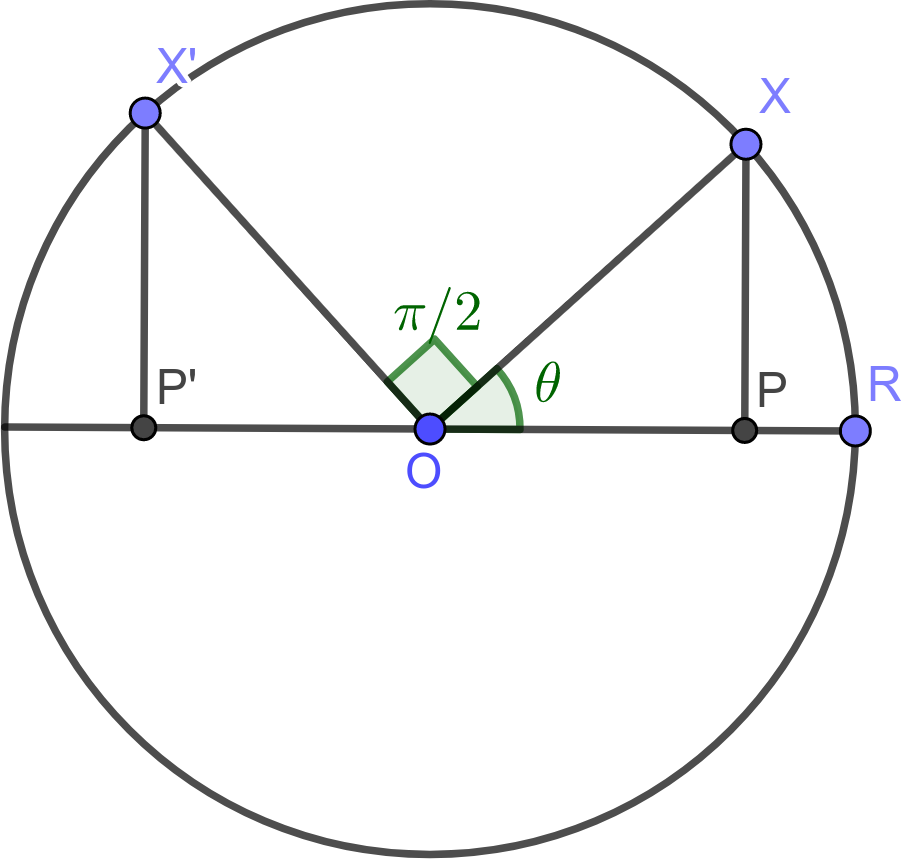
\includegraphics[width=0.3\textwidth]{shifting}
          \end{center}
          The angle $ \angle X'OP' $ has magnitude $ \frac{\pi}{2} - \theta $; hence the other angle in the right
          triangle $ X'OP' $ has magnitude $ \theta $ (since the angle-sum of triangles is $ \pi $). The two triangles
          $ XOP $ and $ X'OP' $ share all three of their angles and so are similar, and share an edge length (the radius
          of the circle) and so are equal, with lengths $ \abs{X'P'} = \abs{OP} $ and $ \abs{OP'} = \abs{XP} $. But $ \abs{X'P'} = \sin(\theta + \pi/2) $,
          and $ \abs{OP} = \cos \theta $; hence the proposition holds in this case.

          If $ \pi/2 \leq \theta < \pi $, then $ \pi \leq \theta + \pi/2 < 3\pi/2 $ and $ \sin(\theta + \pi/2) = -\sin(\theta + \pi/2 - \pi) $;
          then (applying the case we have already proved) $ -\sin(\theta - \pi/2) = -\cos(\theta - \pi) = \cos \theta $ as required. We extend
          the proof to all $ 0 \leq \theta < 2\pi $ using similar arguments, and then conclude it holds for all $ \theta $ by periodicity.
  \end{enumerate}
\end{proof}

\begin{thm}
  If $ ABC $ is a right triangle such that the right angle is at $ C $, and $ \alpha $ is the interior angle at $ A $, then
    \begin{gather}
      \sin \alpha = \frac{\abs{BC}}{\abs{AB}} = \frac{\text{opposite}}{\text{hypotenuse}} \text{ and}\\
      \cos \alpha = \frac{\abs{AC}}{\abs{AB}} = \frac{\text{adjacent}}{\text{hypotenuse}}.
    \end{gather}
\end{thm}
\begin{proof}
  Construct a similar triangle $ A'B'C' $ by scaling every length of $ ABC $ by $ 1/\abs{AB} $; drawing a circle
  with radius 1 and centre $ A $, we see that $ \abs{B'C'} = \cos \alpha $ and $ \abs{A'C'} = \sin \alpha $ (taking
  the base radius to be $ A'C' $ and applying our original definition \ref{defn:trig1}). But $ \abs{B'C'} = \abs{BC}/\abs{AB} $,
  and $ \abs{A'C'} = \abs{AC}/\abs{AB} $, so we are done.
\end{proof}

Instead of pushing the definitions further, we take all the properties we know that sine and cosine have and move on to
defining some more trigonometric functions. Consider the following diagram.

\begin{center}
  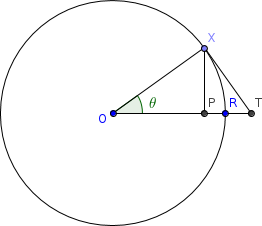
\includegraphics[width=0.3\textwidth]{tangent}
\end{center}

\begin{thm}
  If $ OXP $ is drawn in a unit circle as in the diagram, and the tangent line to the circle at $ X $ is drawn to meet the line $ OR $ at
  some point $ T $, then $ \abs{XT} = \frac{\sin \theta}{\cos \theta} $.
\end{thm}
\begin{proof}
  I claim that $ XOT $ is similar to $ POX $. This is proved by noticing that both triangles
  contain a right angle and share the angle of measure $ \theta $. Hence $ \frac{\abs{XT}}{\abs{XO}} = \frac{\abs{XP}}{\abs{OP}} $;
  but $ \abs{XO} = 1 $, $ \abs{XP} = \sin \theta $, and $ \abs{OP} = \cos \theta $, so we are done.
\end{proof}

Motivated by this theorem, we make the following
\begin{defn}
  The \df{tangent} function is the function $ \tan $ that is defined by
  \begin{displaymath}
    \tan \theta = \frac{\sin \theta}{\cos \theta}
  \end{displaymath}
  for all $ \theta \neq \frac{\pi}{2}n $ where $ n $ is an odd integer (since $ \cos \frac{\pi}{2}n $ is zero for odd $ n $).
\end{defn}

\end{document}
